% !TeX root = ../main-paper.tex
\section{Results}

\subsection{OCR evaluation}

\begin{figure}

\subcaptionbox{}[.5\linewidth]{
\begin{tabular}{rll}
          & CER & CER$_{norm.}$ \\
\midrule
Pero      & 3.78\% & 3.76\% \\   
Tesseract & 6.56\% & 6.45\% \\
\bottomrule
\end{tabular}

\bigskip

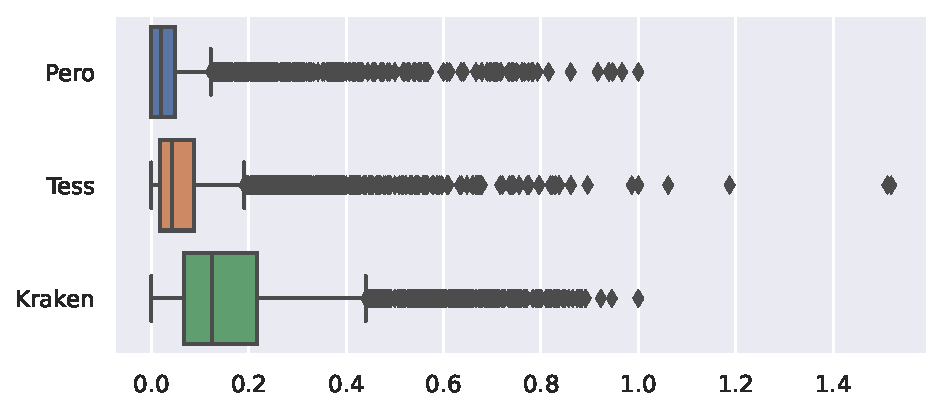
\includegraphics[width=\linewidth]{images/ocr-eval-2.pdf}
}
\subcaptionbox{}[.5\linewidth]{
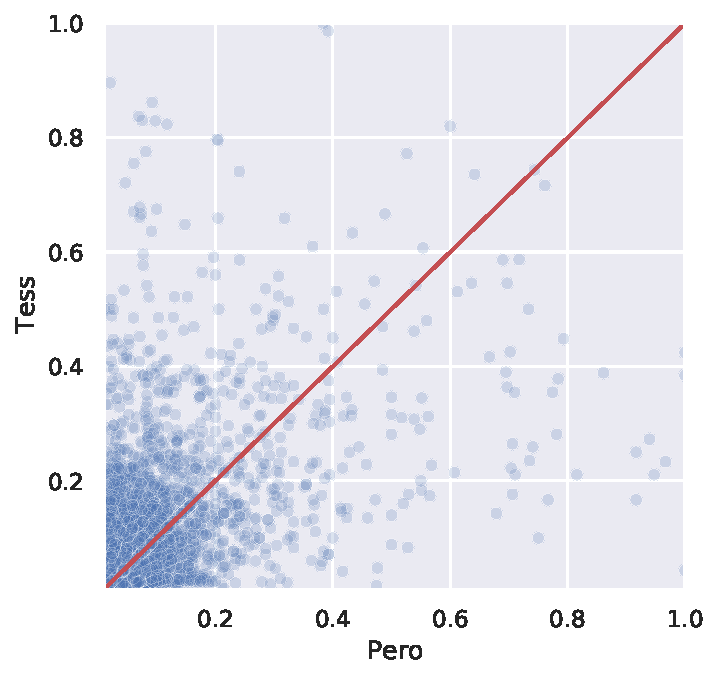
\includegraphics[width=\linewidth]{images/ocr-eval-1.pdf}
}
\caption{Character error rates at entry-level for Pero OCR and Tesseract. (a) Global CER and distribution of the CER per entry. (b):
joint plot of the dataset showing that the two systems do not fail on the same entries.}  
\end{figure}

\subsection{Experiment 1: NER sensibility to the number of training samples}

Qualitative results
\textbf{TODO random samples of results + selection of failure cases}


Quantitative results: table + graph ideally (with training set size info)

\begin{table}[!h]
    \caption{Experimental results of the NER models performances when trained on varying numbers of examples.}
    \centering
    \begin{tabular}{rrrrrrrrrr}
           & Trainset Size &  49   &  99   &  199  &  398  &  796  &  1593 &  3186 &  6373 \\
           & \% & 0.8   & 1.5   & 3.1   & 6.2   & 12.5  & 25.0  & 50.0  & 100.0 \\
    \midrule\bottomrule
    \multirow{3}{*}{\rotatebox{90}{F1 score}} & CamemBERT &  89.6 &  90.1 &  92.8 &  93.4 &  94.3 &  95.3 &  94.7 &  95.5 \\
           & CamemBERT.pretrained &  90.0 &  91.4 &  92.9 &  93.4 &  94.2 &  94.5 &  94.8 &  95.4 \\
           & SpaCy NER &  87.0 &  89.0 &  90.3 &  91.9 &  92.1 &  92.8 &  93.2 &  93.5 \\
    \cline{1-10}
    \multirow{3}{*}{\rotatebox{90}{Precision}} & CamemBERT &  87.8 &  87.8 &  91.7 &  93.0 &  93.4 &  95.4 &  93.8 &  95.8 \\
           & CamemBERT.pretrained &  87.9 &  89.8 &  91.6 &  92.7 &  93.4 &  94.0 &  94.1 &  95.4 \\
           & SpaCy NER &  85.6 &  87.7 &  90.0 &  92.0 &  92.4 &  92.8 &  93.1 &  93.7 \\
    \cline{1-10}
    \multirow{3}{*}{\rotatebox{90}{Recall}} & CamemBERT &  91.5 &  92.5 &  93.9 &  93.9 &  95.2 &  95.1 &  95.6 &  95.1 \\
           & CamemBERT.pretrained &  92.2 &  93.0 &  94.3 &  94.2 &  95.0 &  95.1 &  95.5 &  95.4 \\
           & SpaCy NER &  88.6 &  90.4 &  90.7 &  91.7 &  91.9 &  92.8 &  93.3 &  93.4 \\
    \end{tabular}    
    \label{tab:my_label}
\end{table}


\begin{figure}[htb!]
	   \center{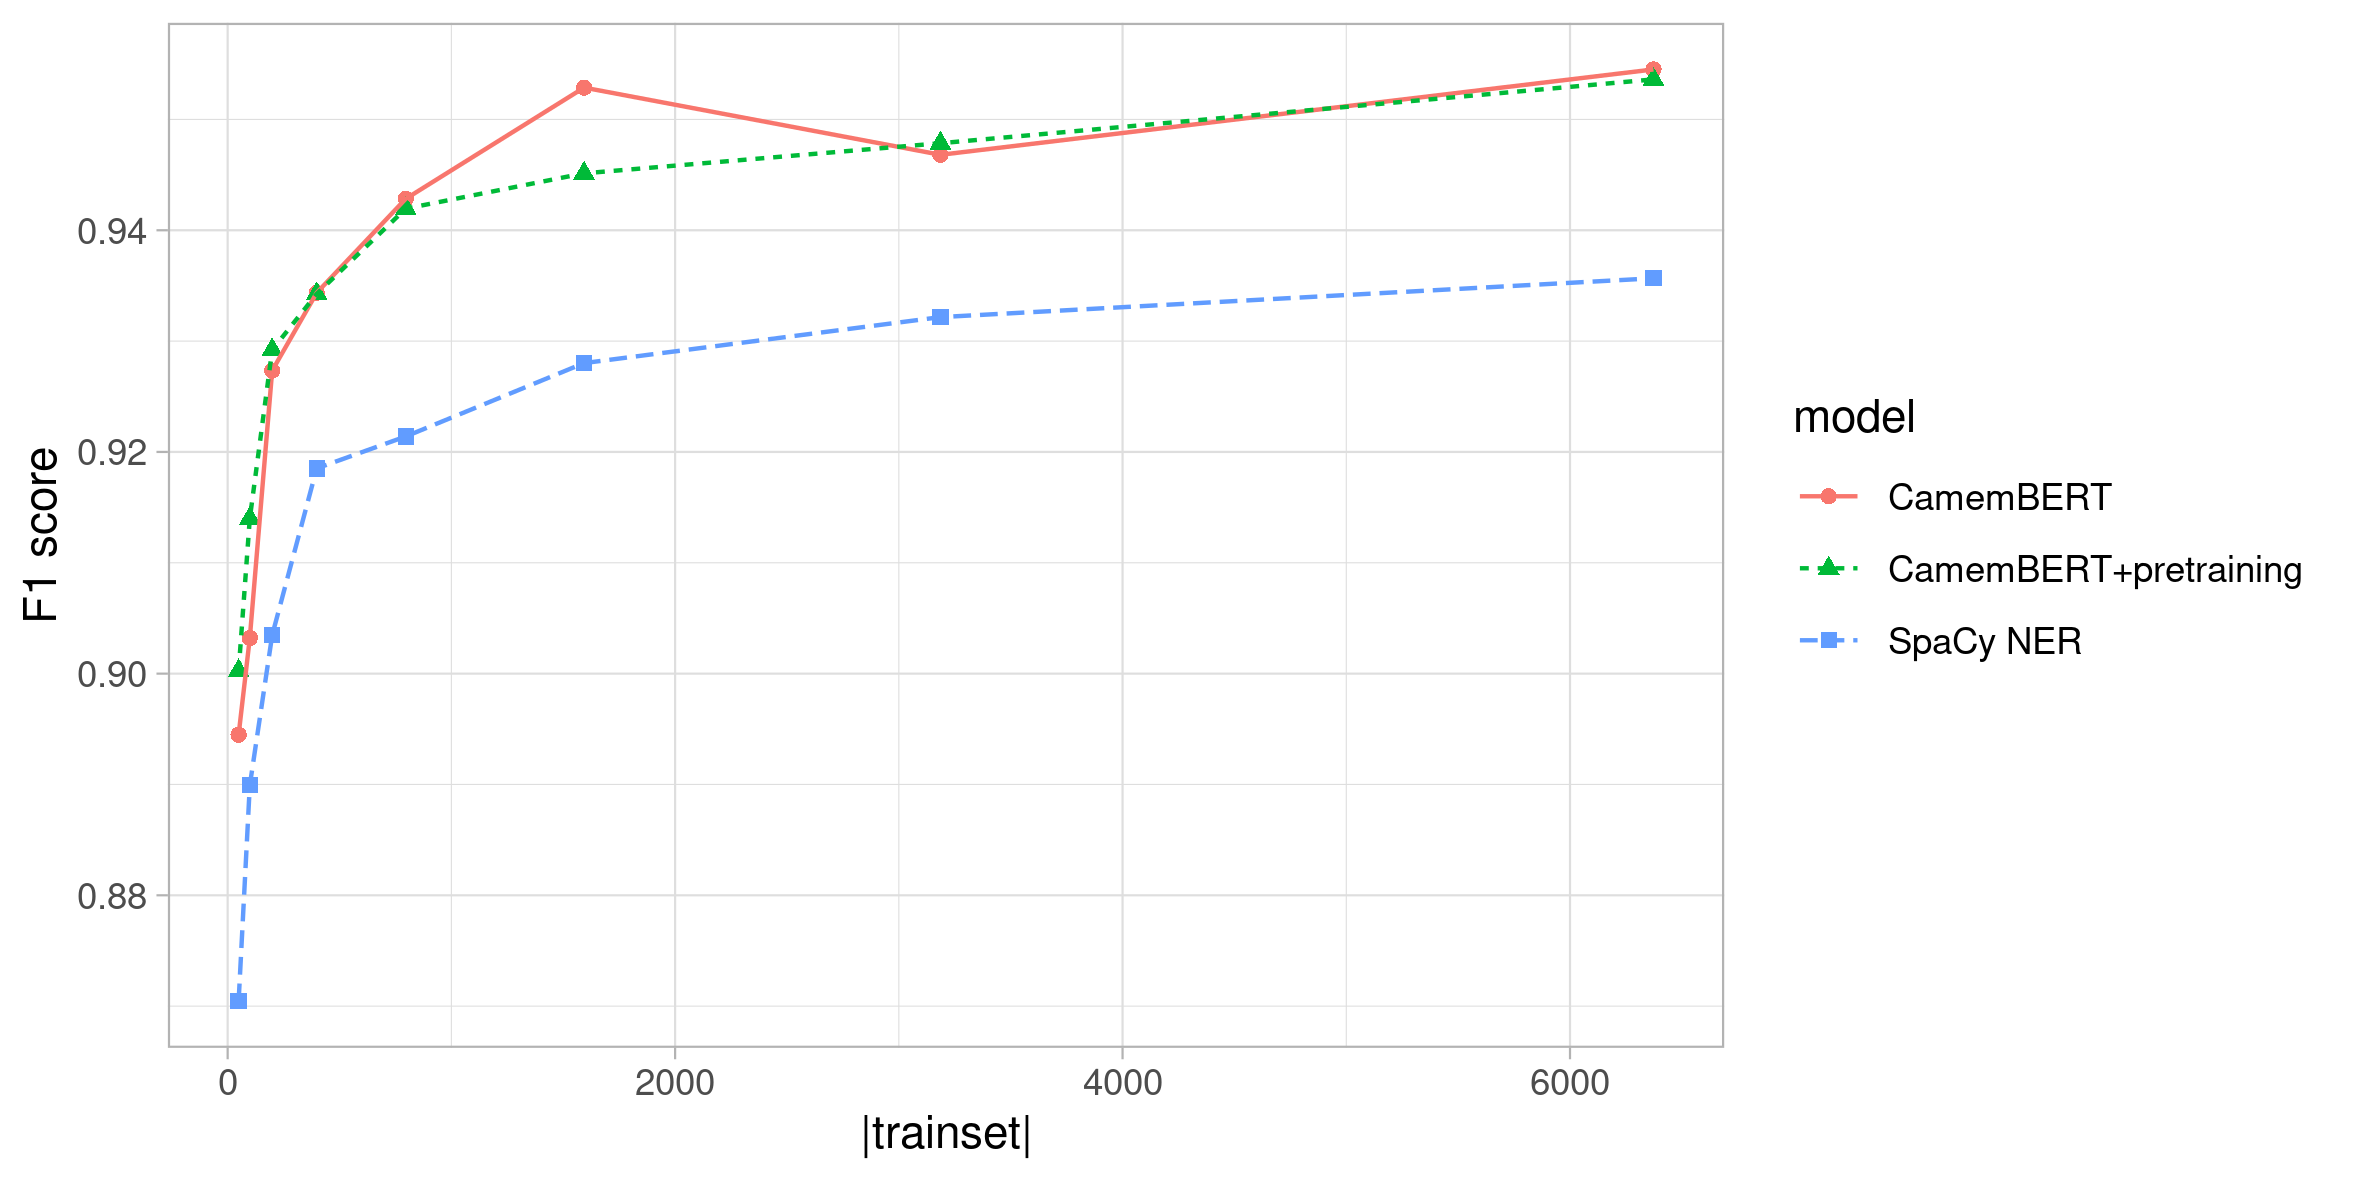
\includegraphics[width=\textwidth]
	       {../material/experiment_1/f1_vs_trainsize.png}}
	  \vspace{3in}
	  \caption{\label{fig:f1-vs-trainsize} Models F1 score on unseen data vs trainset size}
\end{figure}
	                                        


\subsection{Experiment 2: NER in the presence of noisy OCR texts}

Qualitative results
\textbf{TODO random samples of results + selection of failure cases}

Quantitative results: table + graph ideally (with OCR noise, same format as previous)

Table : NER NN models VS train on {noisy, clean} datasets VS evaluate on {noisy, clean} datasets


\begin{table}[h!]
\caption{Camembert vs noise}
\centering
\begin{tabular}{ll|cc|c}
 & & \multicolumn{2}{c|}{Training data} & \\
 & & noisy & clean &   \\ 
\cline{1-4}
\multirow{3}{*}{Test data}& noisy gold (Tesseract) & f1 & f1 & \\
                            & noisy gold (Pero-OCR) & f1 & f1 & \\ 
                            & reference gold & f1 & f1 & \\ 
                            & reference gold & f1 & f1 & \\
\cline{1-4}
\end{tabular}
\end{table}



Opt. use synthetic text perturbation as well? Maybe not interesting and too artificial if we have access to 2+ OCR systems.
(original OCR from BNF, Tesseract 4, Pero OCR…)


\subsection{Discussion}
Interesting points to discuss:
\begin{itemize}
    \item can we train on noisy data? (without manual OCR correction?) => future work? cf Pero OCR training procedure?
    \item do we need better OCR systems or better post-correction techniques (if NER is reliable enough)?
    \item Construction of the lexicon and associated cost
\end{itemize}
